\begin{table}[!t]
\centering
\caption{\textbf{Results of ablation on the feature projector.}}
\label{tab:ablation_projector}
\resizebox{0.48\textwidth}{!}{
\begin{tabular}{l | ccc}
    \toprule
    Projector Arch. & AP & AP$_{50}$ & AP$_{75}$ \\
    \hline
    Baseline & 53.8 & 71.4 & 58.5 \\
    \hline
    w/ 1x1 Conv & 53.8 & 71.5 & 58.5 \\
    w/ MLP & 54.2 & 71.7 & 59.0\\
    w/ Linear & \textbf{54.3} \textcolor{cvprblue}{(+0.5)} & \textbf{71.8} \textcolor{cvprblue}{(+0.4)} & \textbf{59.0} \textcolor{cvprblue}{(+0.5)} \\
    \bottomrule
\end{tabular}
}
\end{table}


\begin{table}[!t]
\centering
\caption{\textbf{Results of ablation on the alignment loss.} The cosine similarity loss demonstrates superior performance. DEIM-M is adopted as the baseline. All reported results are obtained from models trained for 90 epochs with 12 epochs EMA following the training protocol of DEIM.}
\label{tab:ablation_loss}
\resizebox{0.48\textwidth}{!}{
\begin{tabular}{l | ccc}
    \toprule
    Loss Function & AP & AP$_{50}$ & AP$_{75}$ \\
    \midrule
    Baseline & 52.5 & 69.9 & 57.2 \\
    \hline
    w/ MSE Loss & 52.7 & 70.0 & 57.4 \\
    w/ Cosine Similarity & \textbf{53.5} \textcolor{cvprblue}{(+1.0)} & \textbf{71.1} \textcolor{cvprblue}{(+1.2)} & \textbf{58.1} \textcolor{cvprblue}{(+0.9)} \\
    \bottomrule
\end{tabular}
}
\end{table}

\begin{table}[htbp]
\centering
\setlength{\tabcolsep}{4.3pt}
\renewcommand{\arraystretch}{1}
\caption{\textbf{Ablation on the loss weighting strategy.} GAM consistently surpasses the best-tuned static weight. DEIM-L is adopted as the baseline. All reported results are obtained from models trained for 50 epochs with 8 epochs EMA following~\cite{huang2025deim}.}
\label{tab:ablation_gam}
\vspace{-5mm}
\begin{tabular}{c|cccccc}
    \multicolumn{7}{l}{}\\
    \toprule
    $\lambda$ & 0.1 & 0.2 & 0.4 & 1 & 2 & 4 \\
    \arrayrulecolor{gray}\midrule
    AP$^{val}$ & 54.7 & 54.7 & 54.8 & 54.9 & \underline{55.0} & \underline{55.0}  \\
    \arrayrulecolor{black}\midrule[0.8pt]
    $\lambda$ & \underline{10} & \textbf{20} & \underline{30} & 50 & 100 & \textbf{GAM}\\
    \arrayrulecolor{gray}\midrule
    AP$^{val}$ & \underline{55.0} & \textbf{55.1} & \underline{55.0} & 54.9 & 54.6 &  \textbf{55.4} \\
    \arrayrulecolor{black}\bottomrule
\end{tabular}
\end{table}

\begin{figure}[!t]
    \centering
    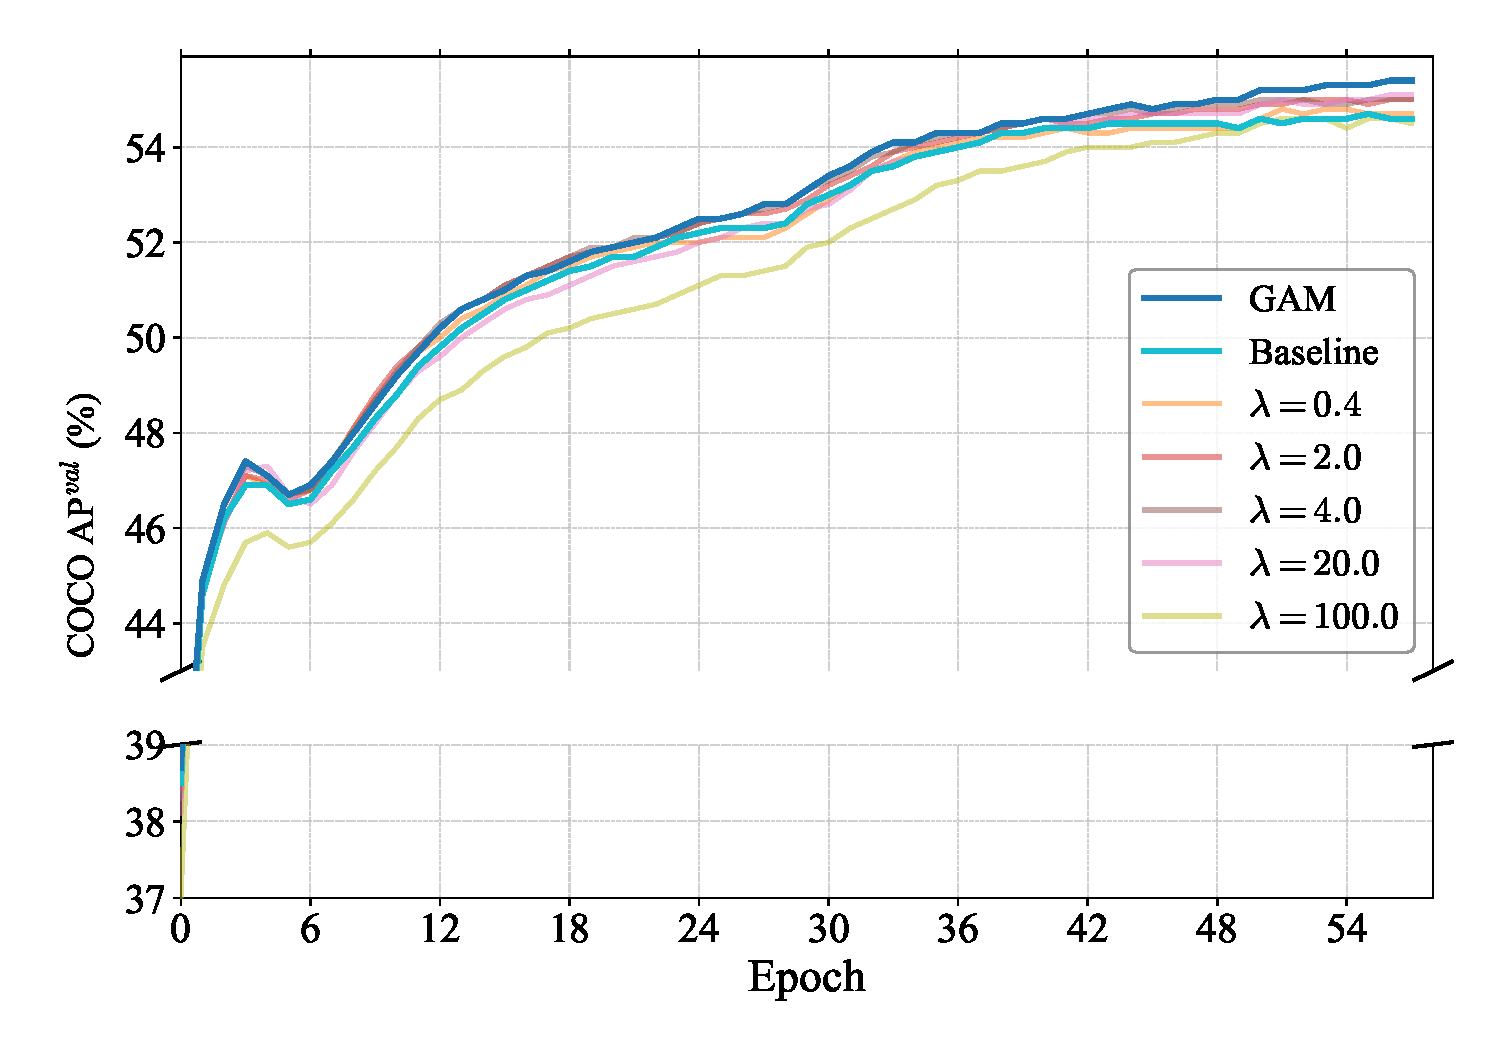
\includegraphics[width=\linewidth]{figures/epoch_vs_ap_broken_axis.pdf}
    \vspace{-5mm}
    \caption{\textbf{Validation AP evolution on COCO during training.} We compare our dynamic GAM with a baseline model and several static $\lambda$ values for the DSI loss. The GAM strategy consistently outperforms all static configurations, showcasing its ability to provide stable and effective supervision throughout the training process.}
    \label{fig:gam_training_curve}
    \vspace{-5mm}
\end{figure}